% Chapter Template

\chapter{NITRO'S INSTALLATION AND MANIPULATION} % Main chapter title

\label{Chapter6} % Change X to a consecutive number; for referencing this chapter elsewhere, use \ref{ChapterX}

\lhead{Chapter 6. \emph{Nitro installation and manipulation}} % Change X to a consecutive number; this is for the header on each page - perhaps a shortened title

%----------------------------------------------------------------------------------------
%	SECTION 1
%----------------------------------------------------------------------------------------

\section{Installation of Nitro}

Pfoh has created a website, \url{http://nitro.pfoh.net/setup.html}, where he gives a general introduction about Nitro’s setup. To reduce the length of this 
report, it’s advised to carefully follow Pfoh’s tutorial when installing Nitro. Here we just provide some extra explanations and complements on the basis 
of his initial tutorial. Remember that Nitro consists of three components:
\begin{itemize}
    \item Kernel Modules - This component is a fork of KVM. It has been extended to provide additional IOCTL calls that can be leveraged to perform VMI.
    \item QEMU - This is a fork of QEMU, the component that provides the user land support for KVM. It is only slightly modified such that it exposes direct access to the guest's physical memory, which Nitro can take advantage of.
    \item Nitro/libnitro - This is the user land component that actually performs VMI. Nitro (this term here represents an executable file/command as opposed to the Nitro project.) calls those APIs defined in libnitro. Remember Nitro is just a prototype implementation which still needs much more enhancements if you want more functionality and could be used as a technique block in other projects. To facilitate possible further work, we have added plenty of comments in Nitro’s source code files. We put Nitro’s source files in path /home/cloud/nitro.
\end{itemize}

%----------------------------------------------------------------------------------------
%	SECTION 2
%----------------------------------------------------------------------------------------

\section{Manipulation of Nitro}

To use Nitro, some preliminary work is necessary, including replace initial KVM modules by a modified one for Nitro, 
mount a huge pages type device under /tmp directory and finally increase the number of huge pages available to your system. 
If you are not familiar with huge pages, this tutorial is a good start point: \url{https://wiki.debian.org/Hugepages}. 
To automate this work, we have written a bash shell script named “load\_mods”, which is located in the root of working directory (/home/cloud/load\_mods). 
If not precise, all script files for Nitro are in the same location. 

Once the huge table file system is set up, QEMU could be launched. 
Note that Nitro uses a modified version of QEMU to directly access the guest's physical memory. 
We put this QEMU in the root of user cloud’s working directory (/home/cloud/qemu). 
When staring the modified QEMU, it works in the same manner as starting vanilla QEMU with KVM support, 
but you must include option “-mem-path [PATH] -mem-prealloc” in the end of QEMU command line. 
It is recommended to use a bash script to automate this work. For example, to start guest with WIN7 OS, 
we write a script named “win7start”.

Finally, it’s time to launch Nitro to monitor the already running VM. We have also a script “NitroStart” for this work. 
Note that Nitro command syntax is “./Nitro PID GUEST\_RAM\_FILE”. Figure \ref{fig:Truncated output of Nitro for a Win7 64bit VM} shows a part of output 
of Nitro.

\begin{figure}[htbp]
	\centering
		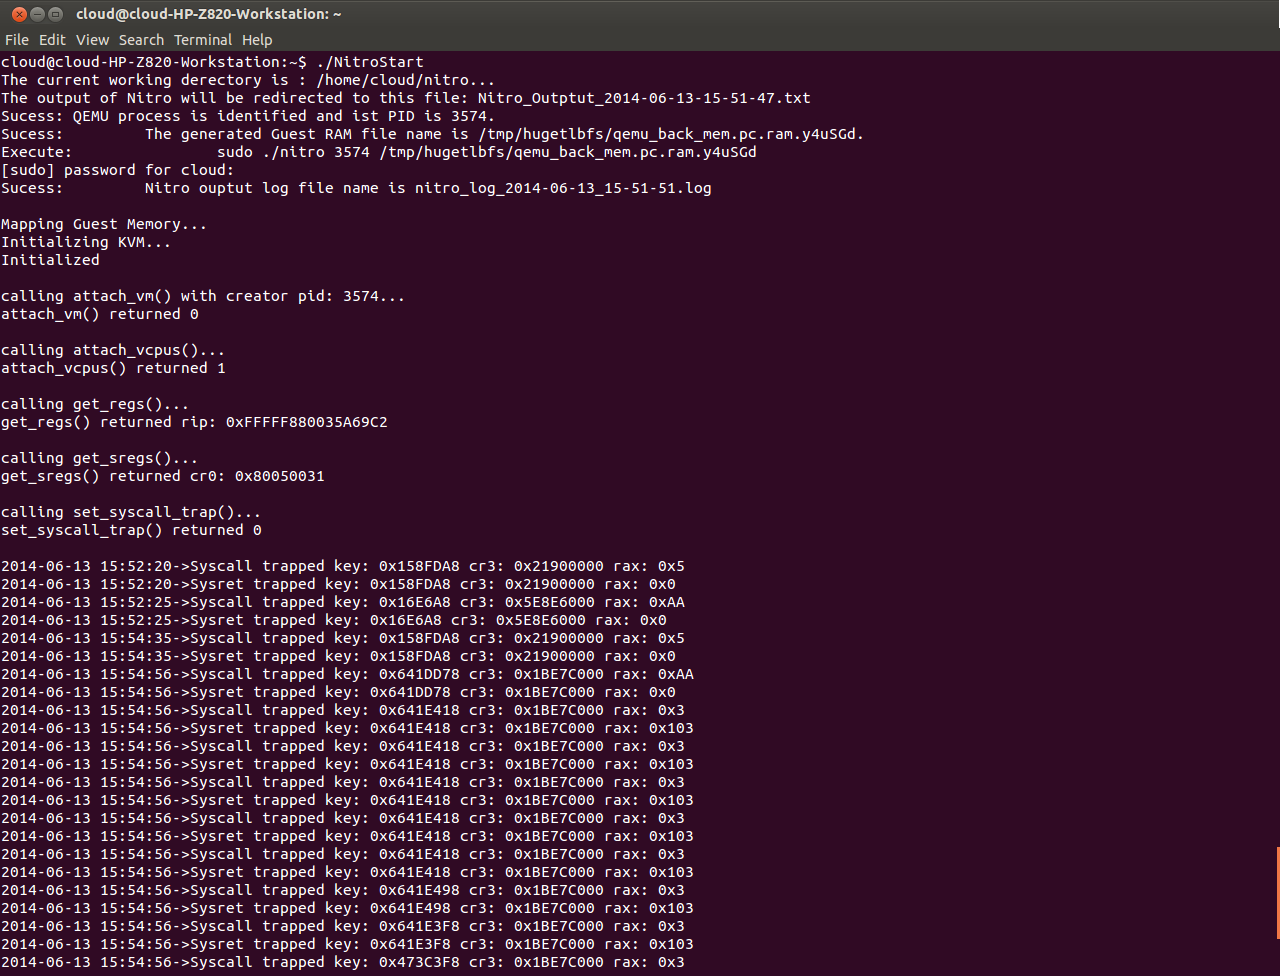
\includegraphics[width=14cm, height= 10cm ]{Figures/Figure19.png}
	\caption[Truncated output of Nitro for a Win7 64bit VM]{Truncated output of Nitro for a Win7 64bit VM}
	\label{fig:Truncated output of Nitro for a Win7 64bit VM}
\end{figure}

All the output of Nitro could be devised into two parties. 
The first part logs the Nitro start process and prints return values for each function invocation. 
For example, function attach\_vcpu( ) returns 1 if Nitro manages to attach to a virtual CPU in guest machine.
(In fact, Nitro now support uniquely attachment to one virtual CPU even if the guest has been allocated more than one virtual CPU.). 
When the invocation of set\_syscall\_trap() returns zero, Nitro is successfully started and ready to capture system call events.
The second part of this output consists of all trapped system call events. Column “Syscall trapped key” means the physical address of 
related system call service routine. Column “cr3” save the CR3 register’s value at the moment of system call trap. And column “rax” 
indicates the system call code for windows 64 bits operating system. For example, a value “AA” in RAX means a system call 
“NtCreateUserProcess” in windows 7. In fact, in the prototype implementation provided by Pfoh, the type of system call desired is 
hard coded in file “nitro\_main.c”. Nitro captures only those system calls that users require.  
For more information about windows 64 bits system call table, please refer to this link: \url{http://j00ru.vexillium.org/ntapi\_64/}.

\section{Assessment of Nitro}
As far as I know, Nitro is actually the first and only VMI application in derivative manner under KVM virtualization platform. 
Though VMI in derivative mode is perfectly against circumstance technique, the amount of information obtained is rather limited, 
due to the fact that derivation method principally just concerns and observes hardware-related running state (such as CR3 register, etc.)
\cite{Reference17}. Nitro, as a typical implementation under the guide of derivation method, is no different. Currently, Nitro is just able to access vCPU 
registers and trap system calls of type “syscall/sysret” (In fact, system call is possible to be invoked in other manners such as assembly instruction int 
0x80.), even though Pfoh promises to enrich Nitro’s functionality list in his spare time.

Just as Pfoh has stated in his project website, Nitro at present has a relatively limited suit of functionalities compared with 
those VMI tools like LibVMI in out-of-band. Concretely, it presents the following limitations:
\begin{itemize}
    \item No documentation about use of Nitro, which is really painful for beginners
    \item No support for AMD CPUs
    \item No support for multi-core guests
    \item Only 64-bit windows guests are supported for now
    \item No cooperation with other tools like virsh/virt-manager
\end{itemize}

The final conclusion for Nitro is that, as a prototype implementation for VMI derivative pattern theory, 
it is a good start point to study, manipulate and modify for the purpose of study, For example, 
to anatomy its modification about KVM modules, we could learn how to enhance KVM virtualization support. As a development framework, 
it is not enough mature to simplify development work, due to the fact Nitro itself is still a project in progress.

The above conclusion could be extended to a conclusion for derivative pattern for VMI application. 
Inferring information from hardware architecture to mitigate semantic gap, this pattern ignores OS-related semantic knowledge to 
get a better portability feature. However, to get high-level information, to implement monitoring task for example, OS-related semantic 
knowledge is somewhat indispensable. We suggest that:

\begin{itemize}
    \item Derivative pattern could be used alongside with Out-of-band pattern to provide a complementary view for guest running state
    \item Derivative is suitable to be used as the last defense line for security purpose
\end{itemize}

\section{Potentialities of CR3 in VMI}
By reading and analyze carefully those VMI applications leveraging CR3 register, we could get some conclusions:

Firstly, the functionality of CR3 register, according to Intel’s specification \cite{BookIntelManuel} and Pfoh’s 
exploiting \cite{Reference17}, is just used to hold the address of the top-level page directory for the currently 
executing process. This value could be used to uniquely represent a process. No others special functionality.
Secondly, the prior work about deriving or inferring guest information from CR3 register is all about countering 
security threats such as identifying hidden processes and stopping them in guest, while our study about CR3 register
is to investigate if CR3 register could provide some information about monitoring network traffic. Accordingly, 
by nature, countering security threats needs less information at the level of process than monitoring task. For 
countering a malicious process, we are allowed to identify the process address space and delete this allocated 
address space to protect guest and it is not necessary to know the PID or process name or application name related 
to the killed dangerous process. However, in the context of monitoring task, for example, monitoring network traffic
on the basis of process, in my view, it needs much more detailed information.


